% convex-polygon-antipodal-diameter.tex

\documentclass[tikz]{standalone}
\usetikzlibrary{calc, positioning}

\begin{document}
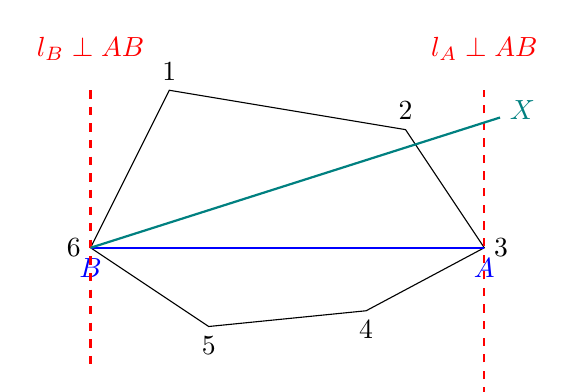
\begin{tikzpicture}
  \coordinate (1) at (1,2); 
  \coordinate (2) at (4, 1.5); 
  \coordinate (3) at (5,0); 
  \coordinate (4) at (3.5, -0.8); 
  \coordinate (5) at (1.5, -1);
  \coordinate (6) at (0,0);

  \path[draw] (6) node[left] {6}
    -- (5) node[below] {5}
    -- (4) node[below] {4}
    -- (3) node[right] {3}
    -- (2) node[above] {2}
    -- (1) node[above] {1}
    -- cycle;

  % A -- B
  \draw[thick, blue] (3) node[below] {$A$} -- (6) node[below] {$B$};

  % \pause
  % l_A, l_B
  \draw[thick, dashed, red, shorten >= -1.5cm, shorten <= -2.3cm] 
    (3) -- node[above = 2.0cm]{$l_{A} \perp AB$} ($(3)!0.5cm!-90:(6)$);
  \draw[thick, dashed, red, shorten >= -1cm, shorten <= -2cm] 
    (6) -- node[above = 2.5cm]{$l_{B} \perp AB$} ($(6)!0.5cm!-90:(3)$);
  
  % \pause
  \node (x) [above right = 1.5cm and 0.2cm of 3, teal] {$X$};

  % \pause
  \draw[thick, teal] (6) -- (x);
\end{tikzpicture}
\end{document}